%#! platex ProgrammersGuideJa
\chapter{テンソル数学}
\label{chap:1}
この章では,
\index{テンソル}%
テンソルとそれらの代数演算について,
また本書におけるそれらの数学表記について記述します.
そして,テンソルおよびテンソル
\index{テンソル!すうがく@数学}%
数学がOpenFOAMにおいて
どのようにプログラムされているかを説明します.



\section{座標系}
\label{sec:1.1}
OpenFOAMは,主に
\index{れんぞくたい@連続体!りきがく@力学}%
連続体力学,
つまり固体・液体・気体の応力や,
これらの物質の変形や流れに関する力学分野の問題
を解くために設計されています.
このためOpenFOAMは,3次元空間と時間,
そして物理的要素のテンソルによる記述に基づいています.
OpenFOAMで使われる
\index{ざひょうけい@座標系}%
座標系は,
\autoref{fig:1.1}に示すような右手系デカルト座標系です.
この座標系は,$Ox$,$Oy$,$Oz$と名づけられた互いに直角な三つの軸から
原点$O$を定義することによって構成されます.
右手系とは,$O$から$Oz$軸のほうを見下ろしたとき,
$Ox$軸上の点から$Oy$軸上の点へと向かう円弧が
時計回りにみえるように定義されます.


\begin{figure}[ht]
 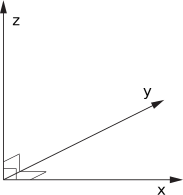
\includegraphics{fig-1-1}
 \caption{右手系座標軸}
 \label{fig:1.1}
\end{figure}



\section{テンソル}
\label{sec:1.2}
テンソル項は,特定の空間に属していて特定の数学的規則に従うような
実体について記述します.
簡潔にいえば,テンソルは単位基底ベクトルの組に対する
成分値の組で表現されます.
OpenFOAMではこの単位基底ベクトルは,
\index{ざひょうじく@座標軸!みぎてけいデカルトざひょうけい@右手系デカルト座標系}%
右手系デカルト座標軸$x$,$y$,$z$にそれぞれ沿った
$\mathbf{e}_{x}$,$\mathbf{e}_{y}$,$\mathbf{e}_{z}$になります.
したがって,これらの基底ベクトルは直交,すなわち互いに直角です.
すべてのテンソルは以下のような属性をもっています.
\begin{description}
 \item[次元] そのテンソルが属する特定の空間の次元$d$.
            OpenFOAMでは$d = 3$
 \item[ランク]
\index{テンソル!ランク}%
            成分値の数が$d^{r}$となるような整数$r \ge 0$
\end{description}
OpenFOAM~1.xが3
\index{テンソル!じげん@次元}%
次元であることから,
ランク$0$〜$3$のテンソルが標準で用意されていますが,
この基本のランクの設定は自由に拡張できるように書かれています.
ランク$0$と$1$のテンソルは,
\index{スカラ}%
スカラおよび
\index{ベクトル}%
ベクトルとしてのほうが
よく知られており読者にも身近でしょうが,
ランク$2$と$3$のテンソルにはあまりなじみがないかもしれません.
確認のために,OpenFOAM~1.xが標準で提供している
すべてのランクのテンソルを以下で復習しておきましょう.
\begin{description}
 \item[ランク0「スカラ」] 一つの実数で表せるあらゆる物理量で,
            イタリック体で表記されます.
            例えば,質量$m$,体積$V$,圧力$p$,そして粘性係数$\mu$です.
 \item[ランク1「ベクトル」] 大きさと方向で表現できる物理量です.
            成分表示では,ベクトル$\bm{a} = (a_{1},\ a_{2},\ a_{3})$は
            デカルト座標系の$x$軸,$y$軸,$z$軸成分をそれぞれ表します.
            同じベクトルを添字表記では$a_{i}$,$i = 1,\ 2,\ 3$と書けます.
            ただし,3次元を扱っていることは明らかなので
            本書では添字リスト$i = 1,\ 2,\ 3$は省略します.
 \item[ランク2「テンソル」] または
\index{テンソル!2かい@2階}%
「2階のテンソル」$\bm{T}$は
            以下のように行列で表現できる9\nobreak 個の要素をもっています.
            \begin{align}
             \label{eq:1.1}
             \bm{T} &= T_{ij}
             = \begin{pmatrix}
                T_{11} & T_{12} & T_{13} \\
                T_{21} & T_{22} & T_{23} \\
                T_{31} & T_{32} & T_{33}
               \end{pmatrix}
            \end{align}
            $r = 2$なので,要素$T_{ij}$は二つの添字で表されます.
            以下では添字のリスト$i,\ j = 1,\ 2,\ 3$は省略します.
            $i = j$の要素は対角要素とよばれ,
            $i \ne j$の要素は非対角要素とよばれます.
            対角要素を交差して要素を入れ替えることにより,
            以下のような$\bm{T}$の
\index{テンソル!てんち@転置}%
            \emph{転置}が得られます.
            \begin{align}
             \label{eq:1.2}
             \bm{T}^{\mathrm{T}} &= T_{ji}
             = \begin{pmatrix}
                T_{11} & T_{21} & T_{31} \\
                T_{12} & T_{22} & T_{32} \\
                T_{13} & T_{23} & T_{33}
               \end{pmatrix}
            \end{align}
            注意:ランク3以上のテンソルが出現することは非常にまれなので,
            多くの場合,ランク2のテンソルは単に「テンソル」とよばれます.
 \item[ランク2(対称)]
\index{テンソル!2かいたいしょう@2階対称}%
            「対称」というのは,対角方向に対称,
            つまり$T_{ij} = T_{ji}$であることを表します.
            この場合$T_{12} = T_{21}$,$T_{13} = T_{31}$,
            $T_{23} = T_{32}$なので,独立な要素は6個だけになります.
            対称テンソルであれば9個より6個の要素を保存するほうがメモリを節約できるので,
            OpenFOAMでは対称テンソルと非対称テンソルを区別して扱います.
            連続体力学において遭遇するほとんどのテンソルは対称です.
 \item[ランク3]
\index{テンソル!3かい@3階}%
            27個の要素をもち,添字表記では$P_{ijk}$と書けますが,
            \autoref{eq:1.1}\hskip\xkanjiskip のように行列表示しようとすると非常に長くなります.
\item[ランク3(対称)]
\index{テンソル!3かいたいしょう@3階対称}%
           ランク3の対称テンソルは,OpenFOAMでは
           $P_{ijk} = P_{ikj} = P_{jik} = P_{jki} = P_{kij} = P_{kji}$として定義されており,
           したがって10個の独立した要素をもちます.
           さらに厳密にいえば,これは相等しい三つのベクトルの外積によってつくられます.
           外積については\autoref{ssec:1.3.4}で述べられています.
\end{description}


\subsection{テンソル表記}
\label{ssec:1.2.1}
本書は,空間3次元と時間からなる複雑な偏微分方程式の問題を扱う,数値連続体力学に関するものです.
まず最初に,簡潔でありながら明確な,方程式の表記方法を導入しておくことが不可欠です.
方程式を追いやすいようにするには,スカラ要素のリストを書くよりも,
それ自体にテンソルの概念が含められた一つのもので表記することが必要です.
加えて,あらゆるテンソル演算が,要素それぞれに体する演算ではなく
テンソル自体に対する演算である,とわかるような表記法であるべきです.

そういうわけで,この文書ではランク1以上のテンソル,
すなわちスカラ以外のすべてのテンソルについては
\index{テンソル!ひょうき@表記}%
\emph{テンソル表記}を採用し,
太字で,例えば$\bm{a}$のように表記します.
これは一つのシンボルで表され,非常にコンパクトであることから,
それ自体で一つの存在としてテンソルを把握しやすくなります.
欠点をあげるとすれば,太字のシンボルはランク0でないことは明らかですが,
そのランクがすぐには読み取れないことです.
しかしながら,シンボルを見れば何の物理量を表しているかがわかり,
直観的にランクもわかるので,実際にはそれほど問題になりません.
例えば,私たちは速度$\bm{U}$がランク1のテンソルであることを知っています.

さらにいえば,表記方法の選択を評価するもっと根本的な点は,
テンソルの数学的表現が座標系によって変化しないこと,
つまりベクトル$\bm{a}$がどこから観測するかに拘らず
同じベクトルであることです.
テンソル表記は,座標系に関する情報をいっさい含まないので,
このコンセプトに合っています.
しかし,他の表記,たとえば$a_{i}$のようにテンソルの成分個別の表示は
必然的に座標系の選択を意味してしまいます.
この望ましくない結果は,
一意でない,つまり座標系に依存する
値の組み合わせでテンソルが表現されることによります.

とはいえ本書では,主にテンソル演算を成分要素に展開するために,
\autoref{sec:1.2}で述べたような添字表記もときどき用います.
添字表記を用いる際には,和の規約を採用します.
これは,一つの項に同じ添字が2回現れたら,
その添字については該当する全ての数字,たとえば$1$,$2$,$3$をとり,
それらの和をとるというものです.
たとえば次のようになります.
\begin{align}
 \label{eq:1.3}
 a_{i}b_{i} = \sum^{3}_{i=1}a_{i}b_{i} = a_{1}b_{1} + a_{2}b_{2} + a_{3}b_{3}
\end{align}

添字が繰り返されたら和を意味するので,この文書では今後,記号$\sum$は省略します.



\section{テンソルの代数演算}
\label{sec:1.3}
この節では,OpenFOAMで利用できるテンソルの
\index{テンソル!だいすうえんざん@代数演算}%
代数演算をすべて紹介します.
まず,もっとも基本的なテンソル演算をおさらいしておきましょう.
\index{テンソル!かさん@加算}%
加算,
\index{テンソル!げんさん@減算}%
減算,そして
\index{テンソル!スカラのじょうさん@スカラの乗算}%
スカラの乗算と除算です.
加算と減算は,可換則と結合則の両方を満たし,
互いにランクの等しいテンソルどうしに限って意味をもちます.
これはテンソルの要素それぞれについて加算・減算を行う操作であり,
たとえば,二つのベクトル$\bm{a}$と$\bm{b}$の差は
\begin{align}
 \label{eq:1.4}
 \bm{a} - \bm{b} = a_{i} - b_{i} = (a_{1} - b_{1},\ a_{2} - b_{2},\ a_{3} - b_{3})
\end{align}
となります.
テンソル$\bm{a}$にスカラ$s$をかける乗算も同様に可換則と結合則を満たし,
テンソルの要素すべてにスカラを乗じる操作です.
たとえば,次のようになります.
\begin{align}
 \label{eq:1.5}
 s\bm{a} = sa_{i} = (sa_{1},\ sa_{2},\ sa_{3})
\end{align}
テンソル$\bm{a}$と
\index{テンソル!スカラのじょさん@スカラの除算}%
スカラの除算は,
スカラが演算の第2引数となっているときにのみ意味をもちます.
つまり,次のとおりです.
\begin{align}
 \label{eq:1.6}
 \frac{\bm{a}}{s} = \frac{a_{i}}{s}
 = \left(\frac{a_{1}}{s},\ \frac{a_{2}}{s},\ \frac{a_{3}}{s}\right)
\end{align}
これ以降の節で述べる上記以外の演算は,
ランク1以上のテンソルどうしの,
さらに複雑な積の組み合わせとなっています.


\subsection{内積}
\label{ssec:1.3.1}
\index{テンソル!ないせき@内積}%
内積は,ランク$r_{1}$と$r_{2}$の任意の二つのテンソルを
ランク$r = r_{1} + r_{2} - 2$のテンソルにする演算です.
ランク3までのテンソルの内積演算を以下に示します.
\begin{itemize}
 \item 二つのベクトル$\bm{a}$と$\bm{b}$の内積は可換であり,
       以下のスカラ$s = \bm{a} \inProd \bm{b}$をつくります.
       \begin{align}
        \label{eq:1.7}
        s = a_{i}b_{i} = a_{1}b_{2} + a_{2}b_{2} + a_{3}b_{3}
       \end{align}
 \item テンソル$\bm{T}$とベクトル$\bm{a}$の内積は
       ベクトル$\bm{b} = \bm{T} \inProd \bm{a}$をつくります.
       これは,見やすいように列ベクトルで書くと,以下のようになります.
       \begin{align}
        \label{eq:1.8}
        b_{i} = T_{ij}a_{j} =
        \begin{pmatrix}
         T_{11}a_{1} + T_{12}a_{2} + T_{13}a_{3} \\
         T_{21}a_{1} + T_{22}a_{2} + T_{23}a_{3} \\
         T_{31}a_{1} + T_{32}a_{2} + T_{33}a_{3}
        \end{pmatrix}
       \end{align}
       もし$\bm{T}$が対称でなければ,
       $\bm{b} = \bm{a} \inProd \bm{T} = \bm{T}^{\mathrm{T}} \inProd \bm{a}$は
       以下のようになり,この演算は可換ではありません.
       \begin{align}
        \label{eq:1.9}
        b_{i} = a_{j}T_{ji} =
        \begin{pmatrix}
         a_{1}T_{11} + a_{2}T_{21} + a_{3}T_{31} \\
         a_{1}T_{12} + a_{2}T_{22} + a_{3}T_{32} \\
         a_{1}T_{13} + a_{2}T_{23} + a_{3}T_{33}
        \end{pmatrix}
       \end{align}
 \item 二つのテンソル$\bm{T}$と$\bm{S}$の内積は,
       以下のような成分をもつテンソル$\bm{P} = \bm{T} \inProd \bm{S}$をつくります.
       \begin{align}
        \label{eq:1.10}
        P_{ij} = T_{ik}S_{kj}
       \end{align}
       これは$\bm{T} \inProd \bm{S} =
       (\bm{S}^{\mathrm{T}} \inProd \bm{T}^{\mathrm{T}})^{\mathrm{T}}$となり,非可換です.
 \item ベクトル$\bm{a}$と3階のテンソル$\bm{P}$の内積は,
       以下のような成分をもつ2階のテンソル$\bm{T} = \bm{a} \inProd \bm{P}$をつくります.
       \begin{align}
        \label{eq:1.11}
        T_{ij} = a_{k}P_{kij}
       \end{align}
       やはりこれも非可換で,
       $\bm{T} = \bm{P} \inProd \bm{a}$は次のようになります.
       \begin{align}
        \label{eq:1.12}
        T_{ij} = P_{ijk}a_{k}
       \end{align}
 \item 2階のテンソル$\bm{T}$と3階のテンソル$\bm{P}$の内積は,
       以下のような成分をもつ3階のテンソル$\bm{Q} = \bm{T} \inProd \bm{P}$をつくります.
       \begin{align}
        \label{eq:1.13}
        Q_{ijk} = T_{il}P_{ljk}
       \end{align}
       やはりこれも非可換で,
       $\bm{Q} = \bm{P} \inProd \bm{T}$は次のようになります.
       \begin{align}
        \label{eq:1.14}
        Q_{ijk} = P_{ijl}T_{lk}
       \end{align}
\end{itemize}


\subsection{二つのテンソルの二重内積}
\label{ssec:1.3.2}
二つの2階テンソル$\bm{T}$と$\bm{S}$の
\index{テンソル!にじゅうないせき@二重内積}%
二重内積は,
スカラ$s = \bm{T} \biInProd \bm{S}$をつくります.
これは,テンソル成分の9個の積の和として得られます.
\begin{align}
 \label{eq:1.15}
 \begin{aligned}
  s = T_{ij}S_{ij} &= T_{11}S_{11} + T_{12}S_{12} + T_{13}S_{13} + {} \\
  &\hphantom{{}={}} T_{21}S_{21} + T_{22}S_{22} + T_{23}S_{23} + {} \\
  &\hphantom{{}={}} T_{31}S_{31} + T_{32}S_{32} + T_{33}S_{33}
 \end{aligned}
\end{align}

2階のテンソル$\bm{T}$と3階のテンソル$\bm{P}$の二重内積は,
次のような成分をもつベクトル$\bm{a} = \bm{T} \biInProd \bm{P}$をつくります.
\begin{align}
 \label{eq:1.16}
 a_{i} = T_{jk}P_{jki}
\end{align}
これは非可換で,$\bm{a} = \bm{P} \biInProd \bm{T}$は次のようになります.
\begin{align}
 \label{eq:1.17}
 a_{i} = P_{ijk}T_{jk}
\end{align}


\subsection{二つの3階テンソルの三重内積}
\label{ssec:1.3.3}
二つの3階テンソル$\bm{P}$と$\bm{Q}$の
\index{テンソル!さんじゅうないせき@三重内積}%
三重内積は,
スカラ$s = \bm{P} \triInProd \bm{Q}$をつくります.
これは,テンソル成分の27個の積の和として得られます.
\begin{align}
 \label{eq:1.18}
 \begin{aligned}
  s = P_{ijk}Q_{ijk}
 \end{aligned}
\end{align}


\subsection{外積}
\label{ssec:1.3.4}
\index{テンソル!がいせき@外積}%
外積は,以下のようなベクトルやテンソルどうしの演算です.
\begin{itemize}
 \item 二つのベクトル$\bm{a}$と$\bm{b}$の外積は非可換で,
       以下のような成分をもつテンソル
       $\bm{T} = \bm{a}\bm{b} = (\bm{b}\bm{a})^{\mathrm{T}}$をつくります.
       \begin{align}
        \label{eq:1.19}
        T_{ij} = a_{i}b_{j} =
        \begin{pmatrix}
         a_{1}b_{1} & a_{1}b_{2} & a_{1}b_{3} \\
         a_{2}b_{1} & a_{2}b_{2} & a_{2}b_{3} \\
         a_{3}b_{1} & a_{3}b_{2} & a_{3}b_{3}
        \end{pmatrix}
       \end{align}
 \item ベクトル$\bm{a}$と2階のテンソル$\bm{T}$との外積は,
       以下のような成分をもつ3階のテンソル
       $\bm{P} = \bm{a}\bm{T}$をつくります.
       \begin{align}
        \label{eq:1.20}
        P_{ijk} = a_{i}T_{jk}
       \end{align}
       これは非可換で,
       $\bm{P} = \bm{T}\bm{a}$は以下のようになります.
       \begin{align}
        \label{eq:1.21}
        P_{ijk} = T_{ij}a_{k}
       \end{align}
\end{itemize}


\subsection{二つのベクトルのクロス積}
\label{ssec:1.3.5}
\index{テンソル!ベクトルのクロスせき@ベクトルのクロス積}%
クロス積はベクトルだけに存在する演算です.
二つのベクトル$\bm{a}$と$\bm{b}$について,
これらのクロス積は以下のような成分をもつベクトル
$\bm{c} = \bm{a} \times \bm{b}$をつくります.
\begin{align}
 \label{eq:1.22}
 c_{i} = e_{ijk}a_{j}b_{k}
 = (a_{2}b_{3} - a_{3}b_{2},\ a_{3}b_{1} - a_{1}b_{3},\  a_{1}b_{2} - a_{2}b_{1})
\end{align}
ここで
\index{ちかんきごう@置換記号}%
\OFemph{置換記号}は以下のように定義されます.
\begin{align}
 \label{eq:1.23}
 e_{ijk} =
 \begin{cases}
  0 & \text{いずれか二つの添字が等しいとき} \\
  +1 & \text{$i,\ j,\ k$が$1,\ 2,\ 3$の偶置換のとき} \\
  -1 & \text{$i,\ j,\ k$が$1,\ 2,\ 3$の奇置換のとき}
 \end{cases}
\end{align}
偶置換とは$123$,$231$および$312$であり,
奇置換は$132$,$213$および$321$です.


\subsection{その他の一般的なテンソル演算}
\label{ssec:1.3.6}
OpenFOAMで使われる,やや一般的でない演算や専門用語を以下に示します.
\begin{description}
 \item[二乗]
\index{テンソル!にじょう@二乗}%
            テンソルの二乗は,それ自身とのテンソル外積で定義されます.
            例えば,ベクトル$\bm{a}$の二乗は$\bm{a}^{2} = \bm{a}\bm{a}$です.
 \item[$n$乗]
\index{テンソル!nじょう@$n$乗}%
            テンソルの$n$乗は,それ自身との$n$回のテンソル外積で定義されます.
            例えば,ベクトル$\bm{a}$の$3$乗は$\bm{a}^{3} = \bm{a}\bm{a}\bm{a}$です.
 \item[平方絶対値]
\index{テンソル!へいほうぜったいち@平方絶対値}%
            テンソルの平方絶対値は,それ自身との$r$テンソルの$r$重内積で,スカラとなります.
            例えば,2階テンソル$\bm{T}$については,$|\bm{T}|^{2} = \bm{T} \biInProd \bm{T}$です.
 \item[絶対値]
\index{テンソル!ぜったいち@絶対値}%
            平方絶対値の平方根です.
            例えば,テンソル$\bm{T}$については,$|\bm{T}| = \sqrt{\bm{T} \biInProd \bm{T}}$です.
            単位長さのベクトルは
\index{ベクトル!たんい@単位}%
            \OFemph{単位ベクトル}とよばれます.
 \item[最大成分]
\index{テンソル!さいだいせいぶん@最大成分}%
            符号も考慮した最大の値をもつテンソルの成分です.つまり最大の絶対値ではありません.
 \item[最小成分]
\index{テンソル!さいしょうせいぶん@最小成分}%
            最小の値をもつテンソルの成分です.
 \item[成分平均値]
\index{テンソル!せいぶんへいきんち@成分平均値}%
            テンソルのすべての成分の平均値です.
 \item[スケール] 名前のとおり,
\index{テンソル!スケールかんすう@スケール関数}%
            スケール関数は,
            あるテンソルの成分を同じランクの他のテンソルの成分でスケーリングします.
            これは二つのテンソルの対応する成分同士の積で評価されます.
            例えば,ベクトル$\bm{a}$のベクトル$\bm{b}$によるスケーリングは,
            以下のような成分のベクトル$\bm{c}$をつくります.
            \begin{align}
             \label{eq:1.24}
             c_{i} = \mathop{\mathrm{scale}}(\bm{a},\ \bm{b})
             = (a_{1}b_{1},\ a_{2}b_{2},\ a_{3}b_{3})
            \end{align}
\end{description}


\subsection{幾何変換と単位テンソル}
\label{ssec:1.3.7}
2階のテンソル$\bm{T}$は線形ベクトル関数,
すなわち,内積$\bm{b} = \bm{T} \inProd \bm{a}$によって,
あるベクトル$\bm{a}$を別のベクトル$\bm{b}$に結びつける関数として,
厳密に定義されます.
$x,\ y,\ z$座標系から新しい座標系$x^{*},\ y^{*},\ z^{*}$への
あるテンソルの座標
\index{テンソル!きかへんかん@幾何変換}%
\index{テンソル!へんかん@変換}%
変換として機能するように,
$\bm{T}$の成分を選ぶことができます.
このとき$\bm{T}$を\OFemph{変換テンソル}とよびます.
スカラは変換によって変化しませんが,
ベクトル$\bm{a}$は
\begin{align}
 \label{eq:1.25}
 \bm{a}^{*} = \bm{T} \inProd \bm{a}
\end{align}
のように$\bm{a}^{*}$に変換されます.
2階のテンソル$\bm{S}$は
\begin{align}
 \label{eq:1.26}
 \bm{S}^{*} = \bm{T} \inProd \bm{S} \inProd \bm{T}^{\mathrm{T}}
\end{align}
に従って$\bm{T}^{*}$に変換されます.

\index{テンソル!たんい@単位}%
\OFemph{単位テンソル}$\bm{I}$は,
あるテンソルをそれ自身に変換するという条件から定義されます.
すべてのベクトル$\bm{a}$に対して
\begin{align}
 \label{eq:1.27}
 \bm{a} = \bm{I} \inProd \bm{a}
\end{align}
となり,つまり
\begin{align}
 \label{eq:1.28}
 \bm{I} = \delta_{ij} =
 \begin{pmatrix}
  1 & 0 & 0 \\
  0 & 1 & 0 \\
  0 & 0 & 1 \\
 \end{pmatrix}
\end{align}
となります.ここで,$\delta_{ij}$は
\index{クロネッカーのデルタ}%
\OFemph{クロネッカーのデルタ}として知られています.


\subsection{便利なテンソルの恒等式}
\label{ssec:1.3.8}
さまざまな
\index{テンソル!こうとうしき@恒等式}%
恒等式を以下に示します.
これらは,関連するすべての微分が存在して連続であるという仮定のもとで証明できます.
スカラ$s$とベクトル$\bm{a}$および$\bm{b}$を用いて表記しています.
%%% 訳注:原文では$\bm{b}$への言及が抜けている.
\begin{align}
 \label{eq:1.29}
 \begin{aligned}
  \nabla \inProd (\nabla \times \bm{a}) &\equiv 0 \\
  \nabla \times (\nabla s) &\equiv \bm{0} \\
  \nabla \inProd (s\bm{a}) &\equiv s\nabla \inProd \bm{a} + \bm{a} \inProd \nabla s \\
  \nabla \times (s\bm{a}) &\equiv s\nabla \times \bm{a} + \nabla s \times \bm{a} \\
  \nabla (\bm{a} \inProd \bm{b})
    &\equiv \bm{a} \times (\nabla \times \bm{b}) + \bm{b} \times (\nabla \times \bm{a})
            + (\bm{a} \inProd \nabla)\bm{b} + (\bm{b} \inProd \nabla)\bm{a} \\
  \nabla \inProd (\bm{a} \times \bm{b})
    &\equiv \bm{b} \inProd (\nabla \times \bm{a}) - \bm{a} \inProd (\nabla \times \bm{b}) \\
  \nabla \times (\bm{a} \times \bm{b})
    &\equiv \bm{a}(\nabla \inProd \bm{b}) - \bm{b}(\nabla \inProd \bm{a})
            + (\bm{b} \inProd \nabla)\bm{a} - (\bm{a} \inProd \nabla)\bm{b} \\
  \nabla \times (\nabla \times \bm{a})
    &\equiv \nabla (\nabla \inProd \bm{a}) - \Laplacian\bm{a} \\
  (\nabla \times \bm{a})
    &\equiv \bm{a} \inProd (\nabla \bm{a}) - \nabla (\bm{a} \inProd \bm{a})
 \end{aligned}
\end{align}
添字表記の数式を操作するときには,
以下の$e$--$\delta$恒等式を知っていると役立つことがあります.
\begin{align}
 \label{eq:1.30}
 e_{ijk}e_{irs} = \delta_{jr}\delta_{ks} - \delta_{js}\delta_{kr}
\end{align}


\subsection{2階テンソル特有の演算}
\label{ssec:1.3.9}
以下に示すように,2階テンソルの成分を操作する様々な演算があります.
\begin{description}
 \item[転置]
\index{テンソル!てんち@転置}%
            \autoref{eq:1.2}で示したように,
            テンソル$\bm{T} = T_{ij}$の転置は$\bm{T}^{\mathrm{T}} = T_{ji}$です.
 \item[対称テンソルと歪(反対称)テンソル] \autoref{sec:1.2}で述べたように,
            $\bm{T} = \bm{T}^{\mathrm{T}}$のように
            成分が対角方向に対称なテンソルを
\index{テンソル!たいしょうテンソル@対称テンソル}%
            対称テンソルとよびます.
\index{テンソル!わいテンソル@歪テンソル}%
            歪テンソルもしくは
\index{テンソル!はんたいしょうテンソル@反対称テンソル|see{歪テンソル}}%
            反対称テンソルは$\bm{T} = -\bm{T}^{\mathrm{T}}$であり,
            当然$T_{11} = T_{22} = T_{33} = 0$となります.
            あらゆる2階テンソルは,以下のように対称テンソルと歪テンソルに分割できます.
            \begin{align}
             \label{eq:1.31}
             \bm{T} = \underbrace{\frac{1}{2}(\bm{T} + \bm{T}^{\mathrm{T}})}_{\text{対称テンソル}}
             + \underbrace{\frac{1}{2}(\bm{T} - \bm{T}^{\mathrm{T}})}_{\text{歪テンソル}}
             = \mathop{\mathrm{symm}}\bm{T} + \mathop{\mathrm{skew}}\bm{T}
            \end{align}
 \item[トレース] テンソル$\bm{T}$の
\index{テンソル!トレース}%
            トレースは対角成分の総和をとったスカラです.
            \begin{align}
             \label{eq:1.32}
             \mathop{\mathrm{tr}}\bm{T} = T_{11} + T_{22} + T_{33}
            \end{align}
 \item[対角] 2階テンソル$\bm{T}$の
\index{テンソル!たいかく@対角}%
            対角成分を成分とするベクトルを返します.
            \begin{align}
             \label{eq:1.33}
             \mathop{\mathrm{diag}}\bm{T} = (T_{11},\ T_{22},\ T_{33})
            \end{align}
 \item[偏差テンソルと静水圧テンソル] あらゆる2階テンソル$\bm{T}$は,
            $\mathop{\mathrm{tr}}T = 0$となる偏差成分と,
            スカラ$s$に対して$\bm{T} = s\bm{I}$となる静水圧成分に分割できます.
            あらゆる2階テンソルは,以下のように
\index{テンソル!へんさテンソル@偏差テンソル}%
            偏差テンソルと
\index{テンソル!せいすいあつテンソル@静水圧テンソル}%
            静水圧テンソルに分割できます.
            \begin{align}
             \label{eq:1.34}
             \bm{T} = \underbrace{\bm{T}
             - \frac{1}{3}(\mathop{\mathrm{tr}}\bm{T})\bm{I}}_{\text{偏差テンソル}}
             + \underbrace{\frac{1}{3}(\mathop{\mathrm{tr}}\bm{T})\bm{I}}_{\text{静水圧テンソル}}
             = \mathop{\mathrm{dev}}\bm{T} + \mathop{\mathrm{hyd}}\bm{T}
            \end{align}
 \item[行列式] 2階テンソルの
\index{テンソル!ぎょうれつしき@行列式}%
            行列式は以下で与えられます.
            \begin{align}
             \label{eq:1.35}
             \begin{split}
              \det\bm{T} &= \begin{vmatrix}
                             T_{11} & T_{12} & T_{13} \\
                             T_{21} & T_{22} & T_{23} \\
                             T_{31} & T_{32} & T_{33}
                            \end{vmatrix} \\
              &= T_{11}(T_{22}T_{33} - T_{23}T_{32})
              - T_{12}(T_{21}T_{33} - T_{23}T_{31})
              + T_{13}(T_{21}T_{32} - T_{22}T_{31}) \\
              &= \frac{1}{6}e_{ijk}e_{pqr}T_{ip}T_{jq}T_{kr}
             \end{split}
            \end{align}
 \item[余因子] テンソルのある成分が属する行と列を取り除いてできた部分を
            $2 \times 2$の行列式として評価したものを,
            テンソルのそれぞれの成分に対する小行列式といいます.
            例えば,$T_{12}$に対する小行列式は
            \begin{align}
             \label{eq:1.36}
             \begin{vmatrix}
              \rlap{\rule[4pt]{67pt}{.4pt}}T_{11} &
              \rlap{\hskip5pt\smash{\rule[-36pt]{.4pt}{44pt}}}T_{12} & T_{13} \\
              T_{21} & T_{22} & T_{23} \\
              T_{31} & T_{32} & T_{33}
             \end{vmatrix}
             = \begin{vmatrix}
                T_{21} & T_{23} \\
                T_{31} & T_{33}
               \end{vmatrix}
             = T_{21}T_{33} - T_{23}T_{31}
            \end{align}
            となります.
\index{テンソル!よいんし@余因子}%
            余因子とは,それぞれの成分の位置に応じて以下のルールで符号付けした小行列式です.
            \begin{align}
             \label{eq:1.37}
             \begin{aligned}
              &\text{$i + j$が偶数ならば$+$} \\
              &\text{$i + j$が奇数ならば$-$}
             \end{aligned}
            \end{align}
            $\bm{T}$の余因子は以下のようになります.
            \begin{align}
             \label{eq:1.38}
             \mathop{\mathrm{cof}}\bm{T} = \frac{1}{2}e_{jkr}e_{ist}T_{sk}T_{tr}
            \end{align}
 \item[逆元]
\index{テンソル!ぎゃくげん@逆元}%
            テンソルの逆元は以下で評価されます.
            \begin{align}
             \label{eq:1.39}
             \mathop{\mathrm{inv}}\bm{T}
             = \frac{\mathop{\mathrm{cof}}\bm{T}^{\mathrm{T}}}{\det\bm{T}}
            \end{align}
 \item[ホッジ双対]
\index{テンソル!ホッジそうつい@ホッジ双対}%
            テンソルのホッジ双対とは,以下のような成分をもつベクトルです.
            \begin{align}
             \label{eq:1.40}
             \mathop{*}\bm{T} = (T_{23},\ -T_{13},\ T_{12})
            \end{align}
\end{description}


\subsection{スカラ特有の演算}
\label{ssec:1.3.10}
OpenFOAMは,スカラを扱うよく知られた関数のほとんどをサポートしています.
例えば平方根,指数,対数,正弦,余弦などで,
これらのリストが\autoref{tbl:1.2}にあります.
OpenFOAMでは,これらに加えて以下の$3$種類の関数も定義されています.
\begin{description}
 \item[符号] スカラ$s$の符号は以下のように得られます.
            \begin{align}
             \label{eq:1.41}
             \mathop{\mathrm{sgn}}(s) =
             \begin{cases}
              1 & \text{$s \ge 0$のとき} \\
              -1 & \text{$s < 0$のとき}
             \end{cases}
            \end{align}
 \item[正数] スカラ$s$に対して以下のように得られます.
            \begin{align}
             \label{eq:1.42}
             \mathop{\mathrm{pos}}(s) =
             \begin{cases}
              1 & \text{$s \ge 0$のとき} \\
              0 & \text{$s < 0$のとき}
             \end{cases}
            \end{align}
 \item[制限] スカラ$s$のスカラ$n$による制限は以下のようになります.
            \begin{align}
             \label{eq:1.43}
             \mathop{\mathrm{limit}}(s,\ n) =
             \begin{cases}
              s & \text{$s < n$のとき} \\
              0 & \text{$s \ge n$のとき}
             \end{cases}
            \end{align}
\end{description}



\section{OpenFOAMのテンソルクラス}
\label{sec:1.4}
OpenFOAMには,これまでに述べたようなテンソル数学のためのクラス群を含んだ
\index{primitive@\OFclass{primitive}!ライブラリ}%
\index{ライブラリ!primitive@\OFclass{primitive}}%
\OFclass{primitive}というC++のクラスライブラリがあります.
OpenFOAMで標準的に使える基本テンソル
\index{テンソル!OpenFOAMにおけるクラス}%
クラスを\autoref{tbl:1.1}に列挙します.
この表にはテンソルの個別の成分にアクセスするための関数,
いわゆる
\index{アクセスかんすう@アクセス関数}%
アクセス関数も列挙してあります.


\begin{table}[ht]
 %#! uplatex ProgrammersGuideJa
\begin{tabular}{clll}
 ランク & 名称 & 基本クラス & アクセス関数 \\
 \hline
 \tblstrut
 $0$ & スカラ &
\index{クラス!scalar@\OFclass{scalar}}%
\index{scalarクラス@\OFclass{scalar}クラス}%
         \OFclass{scalar} & \\
 $1$ & ベクトル &
\index{クラス!vector@\OFclass{vector}}%
\index{vectorクラス@\OFclass{vector}クラス}%
         \OFclass{vector} & \OFkeyword{x()}, \OFkeyword{y()}, \OFkeyword{z()} \\
 $2$ & テンソル &
\index{クラス!tensor@\OFclass{tensor}}%
\index{tensorクラス@\OFclass{tensor}クラス}%
         \OFclass{tensor} & \OFkeyword{xx()}, \OFkeyword{xy()}, \OFkeyword{xz()}, ... \\
 \hline
\end{tabular}

 \caption{OpenFOAMにおける基本テンソルクラス}
 \label{tbl:1.1}
\end{table}


テンソル
\begin{align}
 \label{eq:1.44}
 \bm{T} =
 \begin{pmatrix}
  1 & 2 & 3 \\
  4 & 5 & 6 \\
  7 & 8 & 9
 \end{pmatrix}
\end{align}
は,OpenFOAMでは次の1行で宣言できます.
\begin{OFverbatim}[terminal]
tensor T(1, 2, 3, 4, 5, 6, 7, 8, 9);
\end{OFverbatim}

アクセス関数\OFkeyword{xz()}で
成分$T_{13}$つまり$T_{xz}$にアクセスできます.
例えば,コード
\begin{OFverbatim}[terminal]
Info << ``Txz = '' << T.xz() << endl;
\end{OFverbatim}
は,以下を画面に出力します.
\begin{OFverbatim}[terminal]
Txz = 3
\end{OFverbatim}


\subsection{OpenFOAMにおけるテンソルの代数演算}
\label{ssec:1.4.1}
\autoref{sec:1.3}で述べたすべての
\index{テンソル!OpenFOAMにおけるテンソルのだいすうえんざん@OpenFOAMにおけるテンソルの代数演算}%
代数演算は,
OpenFOAMのテンソルクラスに対して,
数学の表記法によく似た構文で利用できます.
いくつかの関数は,例えば\OFkeyword{symm()}のように,単に記述的な関数で表現しますが,
その他については,例えば\hskip\xkanjiskip\OFkeyword{*}\hskip\xkanjiskip のような演算子記号でも使用できます.
すべての関数を\autoref{tbl:1.2}に列挙します.


\vskip\floatsep
\begingroup
 \small
% \begin{table}[ht]
 \LTXtable{.8\textwidth}{tbl/tbl-1-2}
% 原文では,逆三角関数がプログラミング言語のように
% asin,acos,atan などとされているが,
% あまり数学で使われる表記ではないと思われるため,
% ここでは arcsin,arccos,arctan などとした.
 \addtocounter{table}{-1}%
 \tblcaption{OpenFOAMにおけるテンソルの代数演算}
 \label{tbl:1.2}
% \end{table}
\endgroup
\vskip\floatsep



\section{物理次元の単位}
\label{sec:1.5}
連続体力学では,物理量はある選ばれた単位で記述されます.
例えば,質量はキログラム ($\unit*{kg}$),
体積は立方メートル ($\unit*{m^{3}}$),
圧力はパスカル ($\unit*{kg\,m^{-1}\,s^{-2}}$).
これらの物理量に対する代数演算は,
\index{たんい@単位!けいりょう@計量}%
計量単位を一致させて行わなければなりません.
特に,加算,減算,等価判定は,同じ単位の物理量に対してのみ,物理的な意味をもちます.
無意味な演算の実装を予防するために,
\index{じげん@次元!OpenFOAMにおけるじげんチェック@OpenFOAMにおける次元チェック}%
OpenFOAMはユーザがあらゆるテンソルに物理次元の単位を付加することを推奨し,
これによりあらゆるテンソル演算の際に次元のチェックが行われます.

単位は,例えば以下のように,\OFclass{dimensionSet}クラスで定義されます.
\begin{OFverbatim}[terminal]
dimensionSet pressureDims(1, -1, -2, 0, 0, 0, 0);
\end{OFverbatim}


\begin{table}[ht]
 %#! platex ProgrammersGuideJa
\begin{tabular}{clll}
 No. & 物理量 & 単位 & 記号 \\
 \hline
 \tblstrut
 1 & 質量 & キログラム & $\mathrm{kg}$ \\
 2 & 長さ & メートル & $\mathrm{m}$ \\
 3 & 時間 & 秒 & $\mathrm{s}$ \\
 4 & 熱力学温度 & ケルビン & $\mathrm{K}$ \\
 5 & 物質量 & モル & $\mathrm{mol}$ \\
 6 & 電流 & アンペア & $\mathrm{A}$ \\
 7 & 光度 & カンデラ & $\mathrm{cd}$ \\
 \hline
\end{tabular}

 \caption{SI基本計量単位}
 \label{tbl:1.3}
\end{table}


ここで,それぞれの値は,\autoref{tbl:1.3}に列挙した
SI基本計量単位それぞれの指数を示しています.
このコードでは\OFkeyword{pressureDims}を,
圧力$\unit*{kg\,m^{-1}\,s^{-2}}$の\OFclass{dimensionSet}として宣言しています.
すなわち\OFkeyword{pressureDims}の引数配列の最初の項目$1$は$\unit*{kg^{1}}$を表し,
二つめの$-1$は$\unit*{m^{-1}}$を表す,などのようにです.
単位付きのテンソルは
\index{dimensioned<Type>@\OFclass{dimensioned<Type>}!テンプレートクラス}%
\OFclass{dimensioned<Type>}テンプレートクラスで定義されます.
\OFclass{<Type>}は\OFclass{scalar},\OFclass{vector},\OFclass{tensor}などです.
この
\index{テンプレートクラス!dimensioned<Type>@\OFclass{dimensioned<Type>}}%
\OFclass{dimensioned<Type>}は,
\index{word@\OFclass{word}!クラス}%
\index{クラス!word@\OFclass{word}}%
\OFclass{word}クラスの変数名,
\OFclass{<Type>}の値,そして
\index{クラス!dimensionSet@\OFclass{dimensionSet}}%
\index{dimensionSet@\OFclass{dimensionSet}!クラス}%
\OFclass{dimensionSet}を保持します.

\begin{OFverbatim}[terminal]
dimensionedTensor sigma
    (
        "sigma",
        dimensionSet(1, -1, -2, 0, 0, 0, 0),
        tensor(1e6, 0, 0, 0, 1e6, 0, 0, 0, 1e6),
    );
\end{OFverbatim}
は,圧力あるいは応力としてしかるべき次元をもつ以下のテンソルをつくります.
\begin{align}
 \label{eq:1.45}
 \sigma =
 \begin{pmatrix}
  10^{6} & 0 & 0 \\
  0 & 10^{6} & 0 \\
  0 & 0 & 10^{6} \\
 \end{pmatrix}
\end{align}

